\section{Problem Definition: Proof Repair}
\label{sec:key1}

\toolname is a tool for \textit{proof repair}.
Proof repair is the problem of updating a broken proof in response to a change in a program or specification~\cite{PGL-045, pumpkinpatch}.
We can view this as a form of 
\textit{proof reuse}~\cite{Ringer2019, felty1994generalization, caplan1995logical, pons2000generalization, johnsen2004theorem}, % TODO consider citation list
or reusing proofs about one specification to derive proofs about another specification.
The difference is that in standard proof reuse, both of these specifications continue to exist.
In contrast, proof repair is the process of reusing proofs across \textit{two versions of a single specification},
only one of which---the new version---continues to exist.

\begin{quote}
\textbf{Insight 1}:
Proof repair is a form of proof reuse (Section~\ref{sec:repair}), with the additional
challenge that the specification about which
we are reusing proofs ceases to exist.
The key to supporting proof repair is to build a proof reuse
tool that can handle that additional challenge (Section~\ref{sec:time}).
\end{quote}

\subsection{Repair as Reuse across Equivalences}
\label{sec:repair}

In the \lstinline{list} example from Section~\ref{sec:overview}, \toolname
reused the old proof of \lstinline{rev_app_distr} defined over \lstinline{Old.list}
to generate the new proof of \lstinline{rev_app_distr} defined over \lstinline{New.list}.
Since this change was simple, this required no additional information from the user, and the resulting functions
and proofs behaved exactly the same way.

\begin{figure}
\begin{minipage}{0.48\textwidth}
\codeauto{\lstinputlisting[firstline=1, lastline=15]{equivproof.tex}}
\end{minipage}
\codeauto{\hfill}
\begin{minipage}{0.48\textwidth}
\codeauto{\lstinputlisting[firstline=17, lastline=32]{equivproof.tex}}
\end{minipage}
\caption{Two functions between \lstinline{Old.list} and \lstinline{New.list} (top) that form an equivalence (bottom).}
\label{fig:equivalence}
\end{figure}

More formally, \toolname was able to find a pair of two functions that map between \lstinline{Old.list}
and \lstinline{New.list} and prove that they are mutual inverses, generating the functions and tactic
proofs in Figure~\ref{fig:equivalence} automatically.
\toolname could then use that information to configure its proof term transformation to update
functions and proofs about \lstinline{Old.list} to functons and proofs about \lstinline{New.list} with
the same behavior.

Whenever there exist two functions between two types that are mutual inverses,
there is a \textit{type equivalence}~\cite{univalent2013homotopy} between them, denoted $\simeq$.

\begin{lstlisting}
Old.list $\simeq$ New.list
\end{lstlisting}
Repair corresponds to proof reuse across these equivalences.

\begin{figure}
\begin{minipage}{0.40\textwidth}
   \lstinputlisting[firstline=1, lastline=4]{listtovect.tex}
\end{minipage}
\hfill
\begin{minipage}{0.58\textwidth}
   \lstinputlisting[firstline=6, lastline=9]{listtovect.tex}
\end{minipage}
\caption{A vector (right) is a list (left) indexed by its length.}
\label{fig:listtovect}
\end{figure}

This can support not just simple changes, but also changes in which the proof engineer adds or removes information.
In that case, the equivalence that the tool ports functions and proofs along
is an equivalence between \textit{refinements}.
It is up to the proof engineer to supply the additional information in order to construct proofs about the refinement.
Consider an example from \textsc{Devoid}: changing a list to a length-indexed vector (Figure~\ref{fig:listtovect}).
\textsc{Devoid} is able to repair proofs about lists to proofs about \textit{vectors of some length}, since:

\begin{lstlisting}
list T $\simeq$ $\Sigma$ (n : nat) . vector T n.
\end{lstlisting}
This is enough to automatically repair a lemma about lists:

\begin{lstlisting}
$\forall$ {A B} (l1 : list A) (l2 : list B),
  zip_with pair l1 l2 = zip l1 l2.
\end{lstlisting}
to a lemma about vectors of some length:

\begin{lstlisting}
$\forall$ {A B} (l1 : (@\codediff{$\Sigma$(n : nat).vector A n}@)) (l2 : (@\codediff{$\Sigma$(n : nat).vector B n}@)),
  zip_with pair l1 l2 = zip l1 l2.
\end{lstlisting}
recursively updating dependencies \lstinline{zip} and \lstinline{zip_with}.
It is not enough, however, to help the proof engineer get from that to a proof about vectors \textit{of a particular length}:

\begin{lstlisting}
$\forall$ {A B} (@\codediff{n}@) (l1 : (@\codediff{vector A n}@)) (l2 : (@\codediff{vector B n}@)),
  zip_with pair (@\codediff{n}@) l1 l2 = zip (@\codediff{n}@) l1 l2.
\end{lstlisting}

More desirable is a repair that takes us from lists of a particular length to vectors of that length:

\begin{lstlisting}
$\Sigma$(l : list T).length l = n $\simeq$ vector T n.
\end{lstlisting}
\toolname can handle both of these changes.
Practically, when the proof engineer changes specifications to refer to \lstinline{vector} instead of \lstinline{list},
to fix her functions and proofs, she must additionally prove invariants about the lengths of her lists.
\toolname makes it easy to separate out that proof obligation, and then automates the rest.

\subsection{A Tool for Proof Repair}
\label{sec:time}

The problem of proof reuse across equivalences is known as \textit{transport}. % TODO cite
Thus, any tool that can repair proofs implements transport across the classes
of equivalences that it supports---and so can handle proof reuse as well.
But not every proof reuse tool or transport method can support proof repair.
A proof repair tool must produce proofs
that no longer refer in any way to the old specification, since the old specification no longer exists.

The goal of a proof repair tool is, in essence, to
define a transport method over a broad set of changes that
removes references to the old specification, rather than converting back and forth
like standard transport methods.
For example, the updated proof of \lstinline{rev_app_distr} and its dependencies
from Section~\ref{sec:overview} refer only to \lstinline{New.list} and not to \lstinline{Old.list}.
The proof inducts directly over \lstinline{New.list} and never, at any point, converts to an \lstinline{Old.list}.
Thus, we need \lstinline{Old.list} around only until we call the \lstinline{Repair} command;
after that, we can remove the type and all of the functions and proofs about it, and replace them all with
our functions and proofs about \lstinline{New.list}.

\begin{figure}
\begin{minipage}{0.49\textwidth}
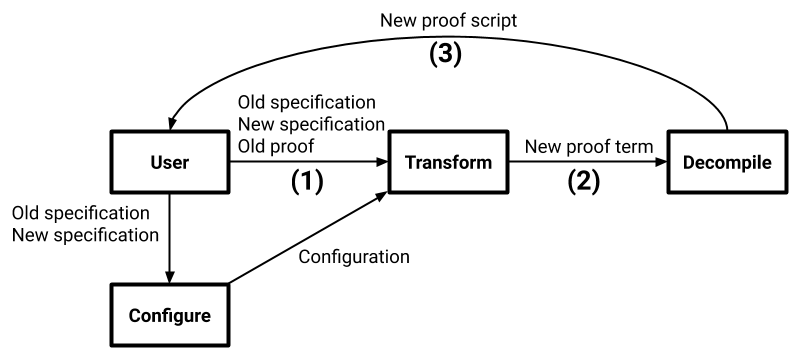
\includegraphics[width=\linewidth]{workflowa.png}
\end{minipage}
\hfill
\begin{minipage}{0.49\textwidth}
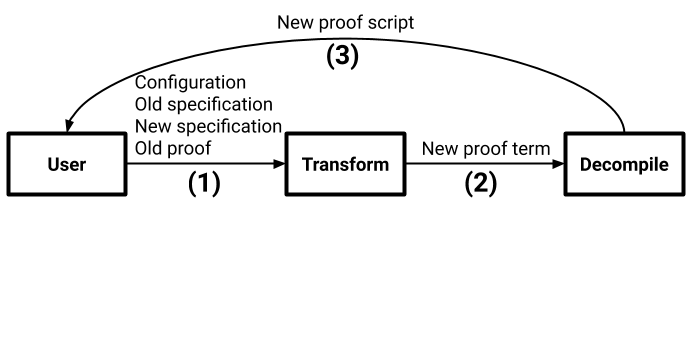
\includegraphics[width=\linewidth]{workflowb.png}
\end{minipage}
\caption{The two possible workflows for \toolname, using either automatic (left) or manual (right) configuration.}
\label{fig:system}
\end{figure}

\toolname accomplishes this using a configurable proof term transformation.
The proof term transformation implements transport across equivalences,
but in a way that replaces references to the old specification (in Section~\ref{sec:overview}, the theorem that refers to \lstinline{Old.list})
with references to the new specification (in Section~\ref{sec:overview}, the theorem that refers to \lstinline{New.list}).
The configuration instantiates the proof term transformation to a particular equivalence corresponding to the old and new 
specifications (in Section~\ref{sec:overview}, \lstinline{Old.list} and \lstinline{New.list}).
Figure~\ref{fig:system} shows how this comes together when the user invokes \toolname:

\begin{enumerate}
\item \toolname configures itself, either:
\begin{enumerate}
\item automatically (left), using \textbf{Configure} to discover the configuration, or
\item manually (right), by taking the configuration as an argument.
\end{enumerate}
\item The configured \textbf{Transform} transforms the old proof term into the new proof term.
\item \textbf{Decompile} produces a new proof script from the new proof term.
\end{enumerate}

The example in Section~\ref{sec:overview} uses automatic configuration. When we run the \lstinline{Repair} command:

\begin{lstlisting}
Repair Old.list New.list in rev_app_distr.
\end{lstlisting}
\textbf{Configure} invokes a special search procedure that automatically discovers that \lstinline{New.list}
is just \lstinline{Old.list} with a single moved constructor.
The search procedure proves an equivalence between \lstinline{Old.list} and \lstinline{New.list},
then configures \textbf{Transform} using that equivalence.
\textbf{Transform} then ports the proof term that inducted over \lstinline{Old.list}
to instead induct over \lstinline{New.list}, and finally
\textbf{Decompile} produces the tactic script that we see.
Section~\ref{sec:search} includes many more examples as applied to real proof reuse and repair scenarios.


